% Liste de paquets potentiellement utiles pour votre rédaction
\documentclass[a4paper, oneside]{report}
\usepackage[french]{babel}      % fonctionnalités en français
\usepackage[utf8x]{inputenc}    % support de l'encodage utf8
\usepackage{listings}           % permet d'insérer du code
\usepackage{hyperref}           % liens
\usepackage{subfigure}          % schémas
\usepackage{amsmath}            % pour ajouter des équations 
\usepackage{graphicx}           % pour \includegraphics 
\usepackage{appendix}           % pour ajouter des appendices à votre rapport
\usepackage[T1]{fontenc}

\usepackage[a4paper,top=2cm,bottom=2cm,left=2cm,right=2cm,marginparwidth=1cm]{geometry} 


% Variables à remplacer :
\newcommand{\anneeUniversitaire}{2020/2021} % 20XX/20XX
\newcommand{\prenomNOM}{CLARY Emilie} % prénom NOM
\newcommand{\dateDebutStage}{14/06/2021} % jour/mois/année
\newcommand{\promo}{CIR 1 - Promotion 66}
\newcommand{\dateFinStage}{09/07/2021 } % jour/mois/année
\newcommand{\nomEntreprise}{Aéroport de Bordeaux-Mérignac}% Nom de l'entreprise en MAJUSCULES
\newcommand{\sujetMission}{Stage Ouvrier} % Sujet de mission
\newcommand{\directeurStage}{CORDEAU Nathalie}
\newcommand{\tuteurEntreprise}{CLARY Serge}
\newcommand{\tuteurEcole}{SAINI Laura}

\begin{document}
% Ajoutez vos sections/chapitres ici
\begin{titlepage}

\newcommand{\HRule}{\rule{\linewidth}{0.5mm}} % épaisseur de lignes horizontales
\setlength\fboxrule{2pt} % épaisseur de la boîte de mission

%----------------------------------------------------------------------------------------
%	SECTION LOGO/ANNEE
%----------------------------------------------------------------------------------------

\begin{tabular}{lr}
    & \begin{minipage}{0.45\textwidth}
    \begin{flushright}
        \Large\textbf{ANNÉE \anneeUniversitaire}
    \end{flushright}
    \end{minipage} \\
    \begin{minipage}{0.45\textwidth}
            
\includegraphics[width=7cm]{Images/junia_isen_logo.jpg}
    \end{minipage}
\end{tabular}

%----------------------------------------------------------------------------------------

\center % centre tout 

%----------------------------------------------------------------------------------------
%	SECTION TITRE
%----------------------------------------------------------------------------------------
\vskip 4em
\Large\textbf{RAPPORT DE STAGE} 
\vskip 1em
par 
\vskip 1em
\textbf{\prenomNOM}
\vskip 1em
{\promo}
\vskip 2em 
Stage Ouvrier
\vskip 1em
Effectué du \dateDebutStage \ au \dateFinStage :
\vskip 2em
Réalisé à l'\textbf{\nomEntreprise}
\vskip 0.5em
\textit{\lieuEntreprise}
\vskip 1.5em

\begin{figure}[hbt!]
    \centering
    
\includegraphics[width=12cm]{Images/Bordeaux_logo.png}
    \label{fig:logoAeroportBordeaux}
\end{figure}

\HRule

%----------------------------------------------------------------------------------------
% SECTION TUTEUR/DIRECTEUR STAGE
%----------------------------------------------------------------------------------------
\vskip 3em
\begin{minipage}[l]{0.95\textwidth}
    \begin{flushleft}
    Directrice de stage : \textbf{\directeurStage}
    \vskip 1em
    Tuteur Entreprise : \textbf{\tuteurEntreprise}
    \vskip 1em
    Tutrice École : \textbf{\tuteurEcole}
    \end{flushleft}
    \vskip 1em
\end{minipage}

%----------------------------------------------------------------------------------------
% SECTION BAS DE PAGE
%----------------------------------------------------------------------------------------

\vfill % remplit le reste de la page avec des espace

\end{titlepage}


\tableofcontents
\newpage
\section*{Introduction}
\addcontentsline{toc}{section}{Introduction}

\subsection{Demande de stage}

Lorsque l'ISEN a élargi les critères de recherche de stage aux "Petits travaux d'informatiques", je me suis tournée vers de nouvelles entreprises qui auraient besoin d'aide sur de la remise à niveau ou des installations de postes.

J'ai finalement réalisé mon stage à l'Aéroport de Bordeaux-Mérignac, et plus précisément au sein du Département des Opérations Techniques.

Pour l'obtention de ce stage, j'ai été mise en relation avec la directrice du secteur informatique de ce département, Madame Nathalie CORDEAU, afin de réaliser un entretien à distance. 

Après l'entretien, j'ai été recontactée pour me donner son accord et discuter des dates de stage.

\subsection{Objectifs par l'ISEN}

Ce stage ouvrier avait pour but de nous faire découvrir le monde de l'entreprise et d'être placé en bas de l'échelle de celle-ci. Il fallait que l'on se rende compte de ce qu'est la hiérarchie et le fonctionnement d'une entreprise dans le monde de la production, dans mon cas de la production de services.

\subsection{Objectifs personnels}

Mes objectifs personnels de ce stage étaient axés autour de deux parties : Satisfaire mes supérieurs, et laisser une empreinte positive de mon passage.

En effet, l'aéroport étant un bassin d'emploi assez conséquent et varié, cela pourrait m'apporter un futur emploi ou stage au sein de cette entreprise.

J'espère avoir réussi cet objectif, mais dans l'ensemble mes supérieurs m'ont fait des retours positifs sur mon travail.

\chapter{Description}

\section{Structure d'accueil}

J’ai donc effectué mon stage au sein du Département des Opérations Techniques (DOT) de l’aéroport de Bordeaux-Mérignac.

La Société Anonyme Aéroport De Bordeaux-Mérignac (SA ADBM) est une entreprise privée à capitaux et actionnaires publics.\newline

Contrairement à ce que l’on pourrait penser, les clients de l’aéroport ne sont pas les passagers, mais les compagnies aériennes. La SA ADBM fournit les infrastructures aux compagnies aériennes en s’assurant du bon déroulement de toutes les opérations : entretien des pistes permettant les atterissages et décollages, gestion des bagages, des passagers, de la sûreté\footnote{Sûreté : Prévenir et lutter contre la malveillance} et de la sécurité\footnote{Sécurité : Prévenir et lutter contre les accidents}. Les passagers sont les clients des compagnies aériennes.\newline

L’aéroport travaille en collaboration avec :


\begin{itemize}
  \item Douane
  \item Police Aux Frontières (PAF)
  \item Gendarmerie des Transports Aériens (GTA)
  \item Direction Générale de l'Aviation Civile (DGAC)
  \item Société de sûreté (HUBSAFE)
  \item Société de sécurité (LYNX)
  \item Société de nettoyage (ONET)\newline
\end{itemize}


\subsection{Un peu d'histoire}

L'aéroport a été construit en 1912 après l'achat de 45 hectares par l'état mais l'aérogare ne connaîtra son premier visage que dans les années 1930.

\begin{figure}[hbt!]
    \begin{subfigure}{0.5\textwidth}
      \centering
      % include first image
      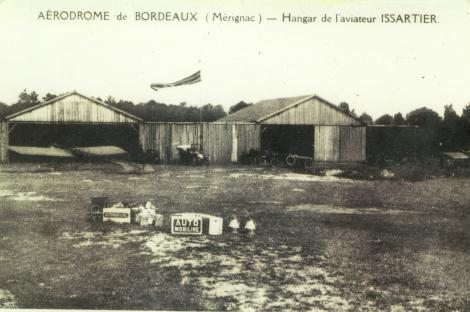
\includegraphics[width=8.5cm]{Images/premier.jpg}  
      \caption{Aérodrome de Bordeaux-Mérignac}
      \label{fig:aérodrome}
    \end{subfigure}
    \begin{subfigure}{0.5\textwidth}
      \centering
      % include second image
      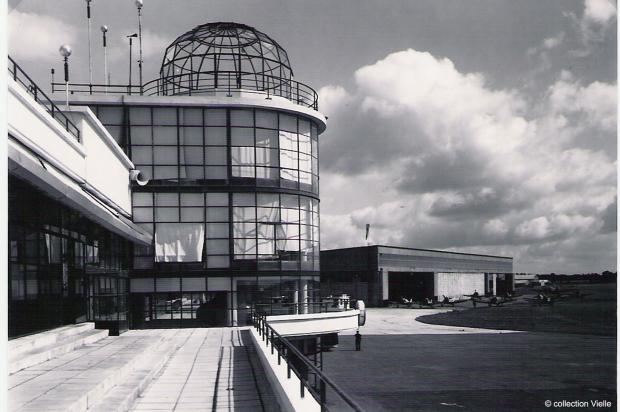
\includegraphics[width=8.5cm]{Images/premiere_aerogare.jpg}  
      \caption{Première aérogare}
      \label{fig:premiereAerogare}
    \end{subfigure}
\end{figure}


\newpage

De nombreux travaux se succèdent jusqu'en 2003 afin d'agrandir l'aéroport. De nouveaux halls d'enregistrement et d'embarquement ainsi qu'une nouvelle tour de contrôle sont ajoutés.

En 2007, l'état concède l'exploitation et la gestion de l'aéroport à la SA ADBM pour 30 ans. Depuis, de nouvelles infrastructures ont été réalisées comme la création d'un nouveau parking passagers plus économique et le hall "billi" destiné aux compagnies aériennes low-cost (Ryanair et EasyJet). Il sera par la suite agrandi en 2015.\newline

\begin{figure}[hbt!]
    \begin{subfigure}{0.5\textwidth}
      \centering
      % include first image
      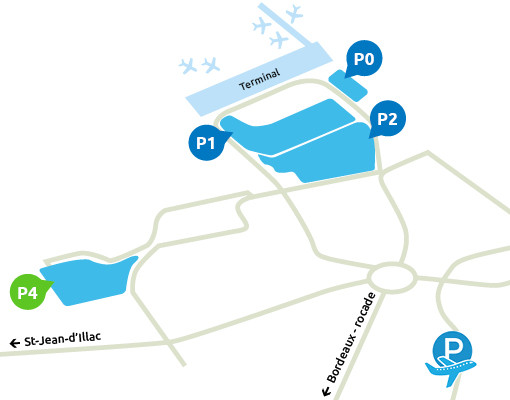
\includegraphics[width=7cm]{Images/parkings.jpg}  
      \caption{Plan des parkings}
      \label{fig:parking4}
    \end{subfigure}
    \begin{subfigure}{0.5\textwidth}
      \centering
      % include second image
      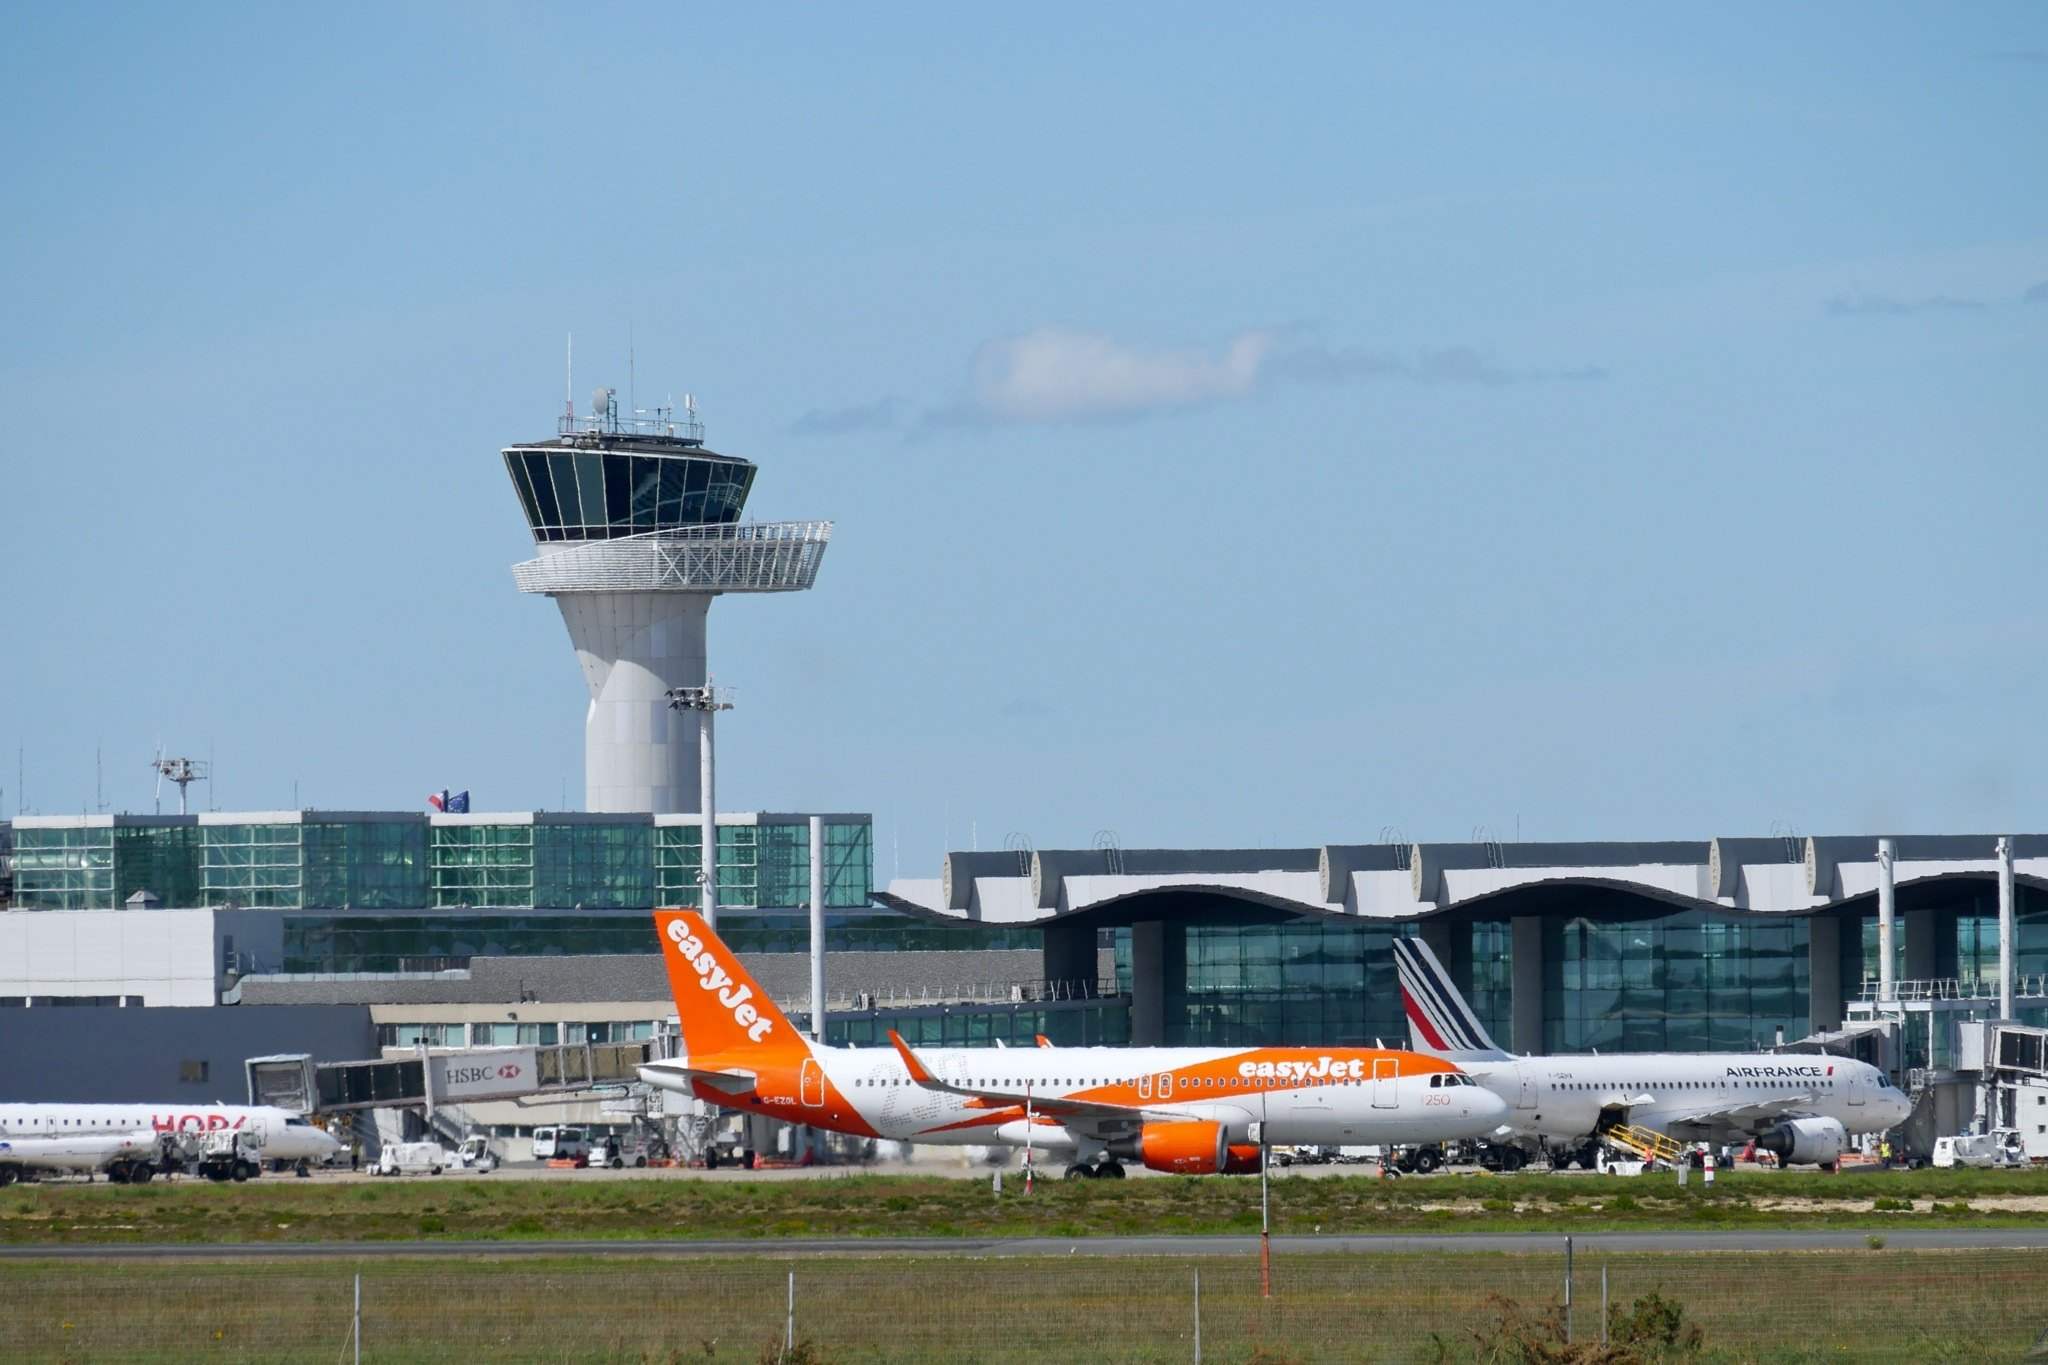
\includegraphics[width=7cm]{Images/tour.jpg}  
      \caption{Nouvelle tour de contrôle}
      \label{fig:tour}
    \end{subfigure}
        
    \begin{subfigure}{.5\textwidth}
      \centering
      % include third image
      
\includegraphics[width=6cm]{Images/billiext.jpg}  
      \caption{Terminal billi}
      \label{fig:billiext}
    \end{subfigure}
    \begin{subfigure}{.5\textwidth}
      \centering
      % include fourth image
      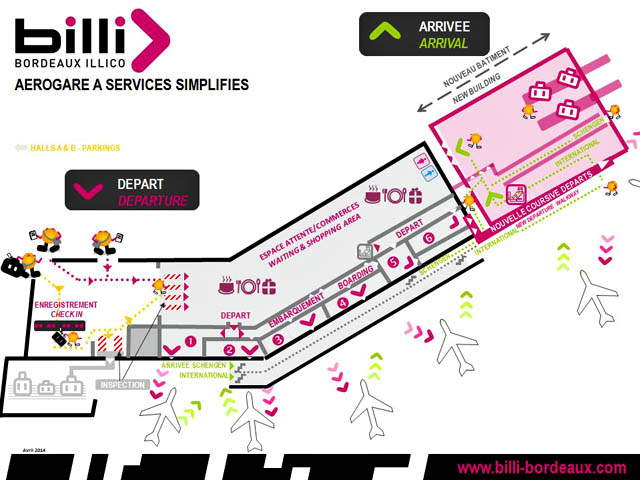
\includegraphics[width=7.5cm]{Images/billi.jpg}  
      \caption{Plan billi}
      \label{fig:planBilli}
    \end{subfigure}
    \label{fig:travaux}
\end{figure}

L’Aéroport de Bordeaux dispose de deux pistes sécantes orientées Nord-Est/Sud-Ouest (piste 05/23) et Sud-Est/Nord-Ouest (piste 11/29). Les trajectoires à l’arrivée et au départ vont dépendre de nombreux paramètres tels que la piste en service, les procédures aériennes, les conditions météo et la typologie des aéronefs.\newline

\begin{figure}[hbt!]
  \centering
  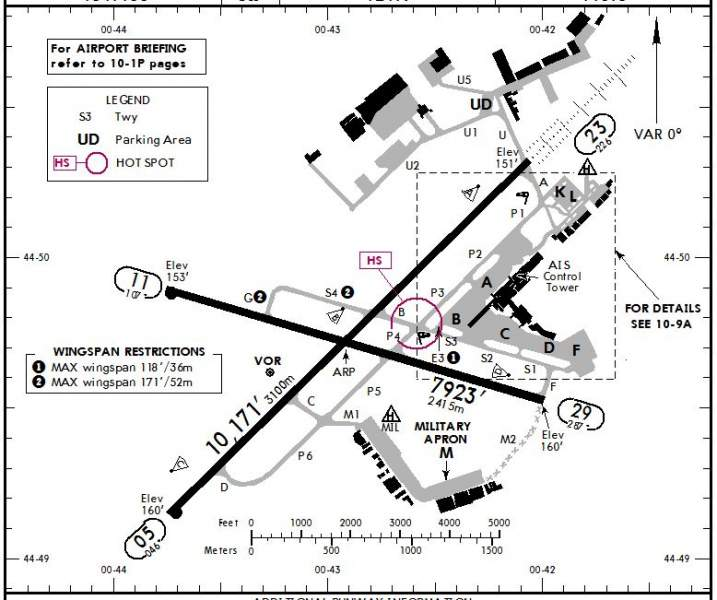
\includegraphics[width=8.5cm]{Images/pistes.jpg}
  \caption{Plan des pistes}
  \label{fig:pistes}
\end{figure}

\newpage

\subsection{Infrastructures actuelles}


A ce jour, la SA ADBM gère et exploite toujours l'aéroport de Bordeaux-Mérignac.
La plateforme aéroportuaire possède 2 pistes sécantes, 39 portes d'embarquements et 3 terminaux :

\begin{itemize}
    \item Le Hall A : National et international
    \item Le Hall B : National
    \item billi : National et international low-cost uniquement (EasyJet et Ryanair)\newline
\end{itemize}

Les Halls A et B possèdent deux niveaux accessibles au public, le niveau 0 pour les arrivées et le niveau 1 pour les départs.

\begin{figure}[hbt!]
    \begin{subfigure}{0.5\textwidth}
      \centering
      % include first image
      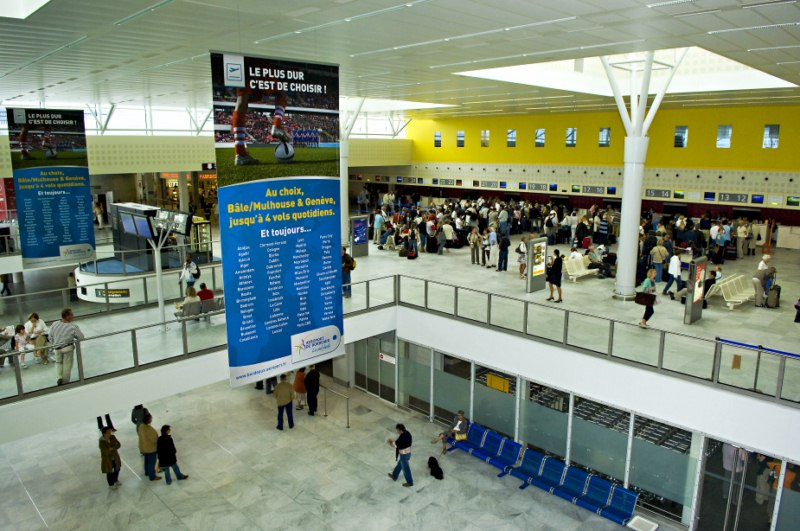
\includegraphics[width=7cm]{Images/inthalla.jpg}  
      \caption{Intérieur Hall A}
      \label{fig:inthalla}
    \end{subfigure}
    \begin{subfigure}{0.5\textwidth}
      \centering
      % include second image
      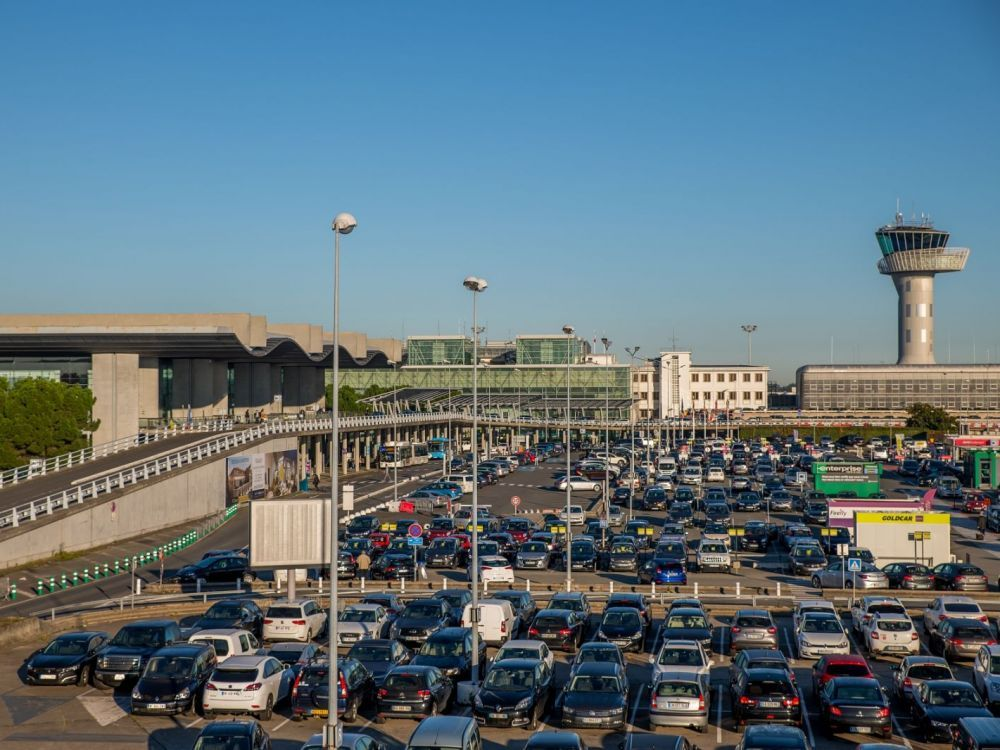
\includegraphics[width=7cm]{Images/exthalla.jpg}  
      \caption{Extérieur Hall A}
      \label{fig:exthalla}
    \end{subfigure}
        
    \begin{subfigure}{.5\textwidth}
      \centering
      % include third image
      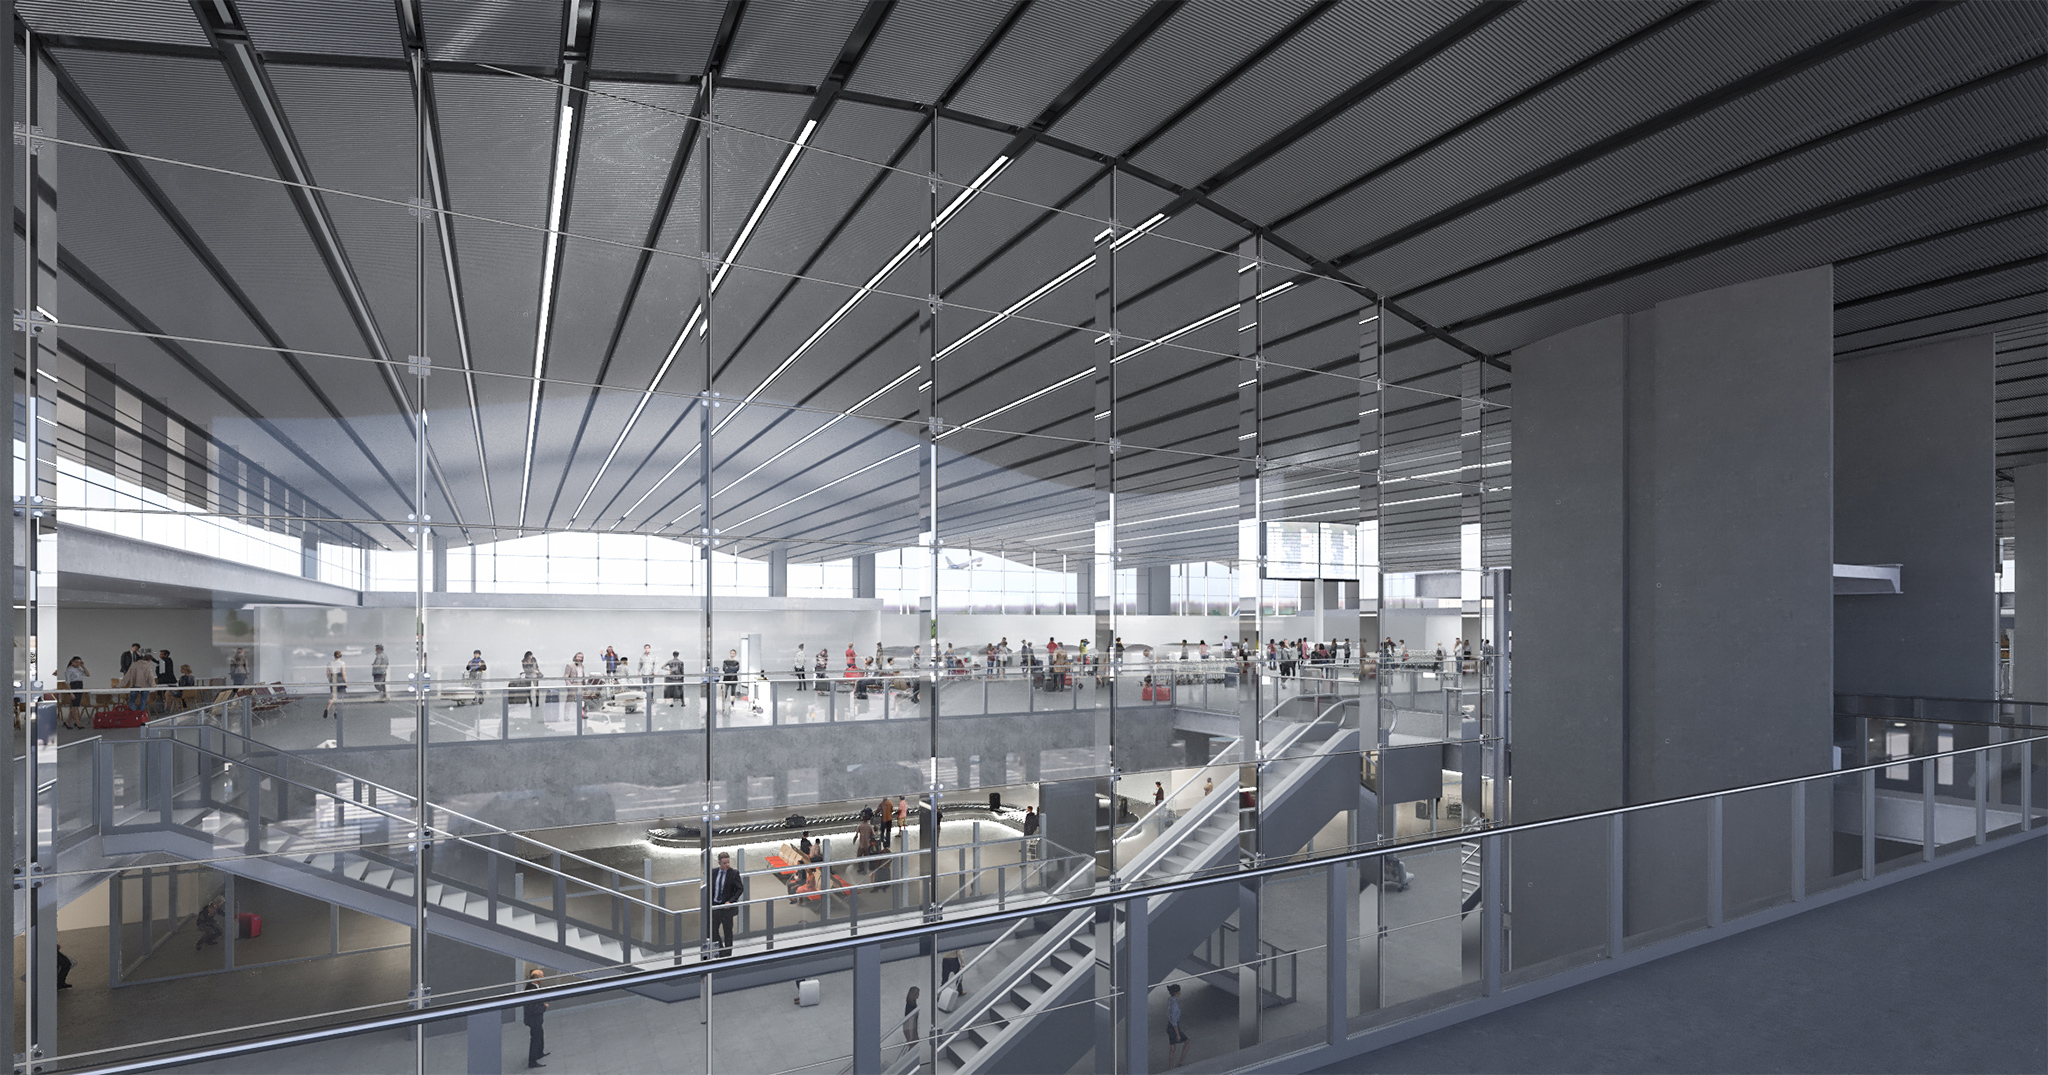
\includegraphics[width=7cm]{Images/inthallb.jpg}  
      \caption{Intérieur Hall B}
      \label{fig:inthallb}
    \end{subfigure}
    \begin{subfigure}{.5\textwidth}
      \centering
      % include fourth image
      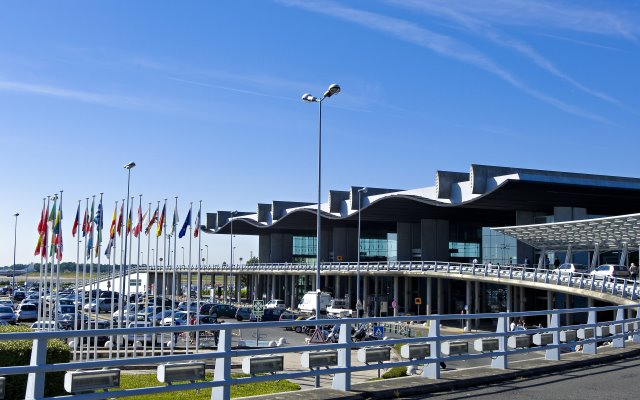
\includegraphics[width=7cm]{Images/exthallb.jpg}  
      \caption{Extérieur Hall B}
      \label{fig:exthallb}
    \end{subfigure}
    \caption{Les différents Halls}
    \label{fig:halls}
\end{figure}

\begin{figure}[hbt!]
    \centering
    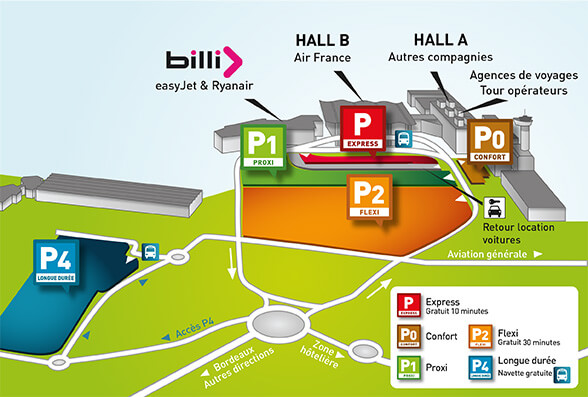
\includegraphics[width=11.2cm]{Images/plan.jpg}
    \caption{Plan général}
    \label{fig:plangeneral}
\end{figure}

\newpage

\subsection{Infrastructures futures}

Actuellement, deux plans d'aménagement ont été engagés : le Satellite 3 et le prolongement de la ligne A du tramway.

Le Satellite 3 est un nouveau bâtiment construit côté piste du Hall A afin d'augmenter le nombre de portes d'embarquement pour l'international.

La livraison de ce bâtiment est prévue pour le 13 août 2021.\newline

\begin{figure}[hbt!]
    \centering
    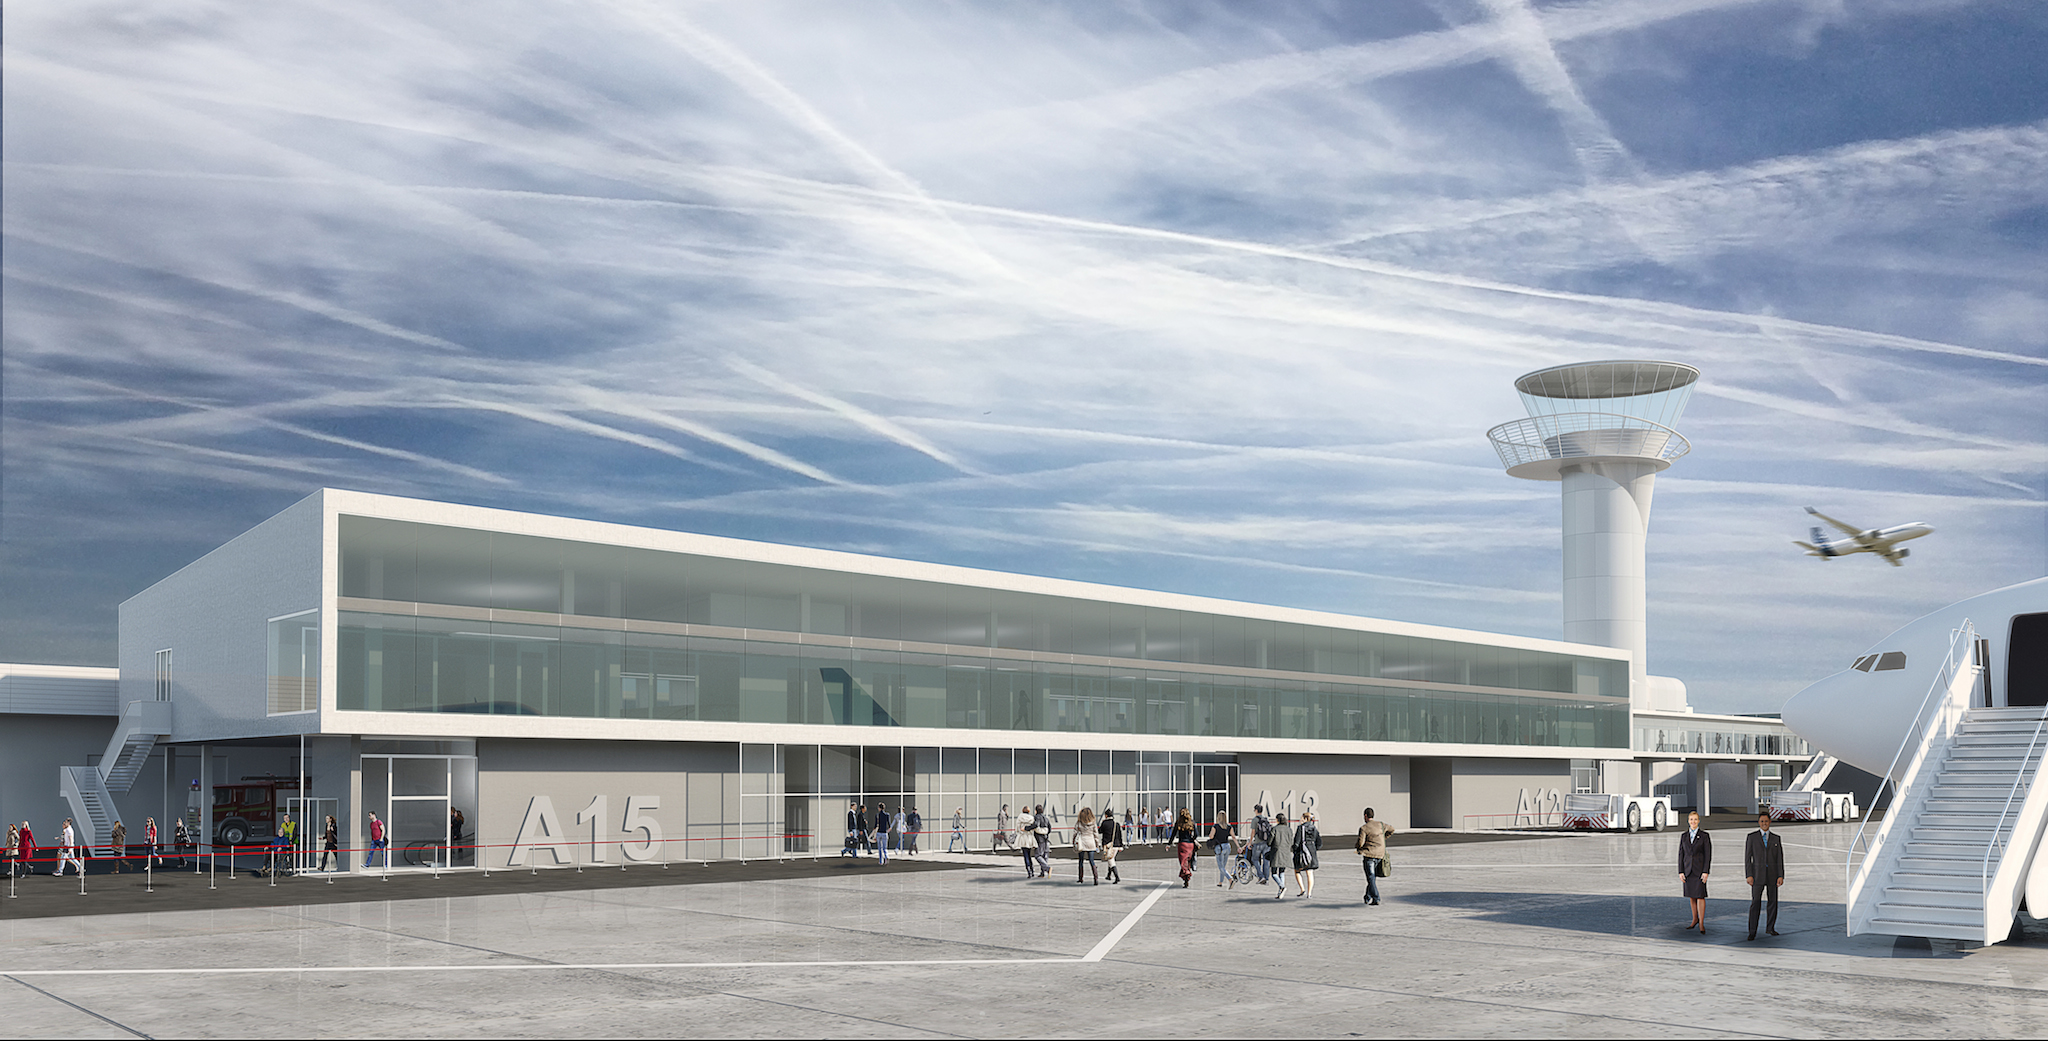
\includegraphics[width=13cm]{Images/satellite3.jpg}
    \caption{Futur Satellite 3}
    \label{fig:sat3}
\end{figure}

En partenariat avec Bordeaux Métropole, la SA ADBM a engagé des travaux qui visent à rendre l'accès à l'aéroport plus simple. La ligne de tramway A est donc prolongée de 6 stations avec le terminus au pied des aérogares. Ces travaux ont été lancés en 2019 et la livraison est prévue pour l'automne 2022.\newline

\begin{figure}[hbt!]
    \centering
    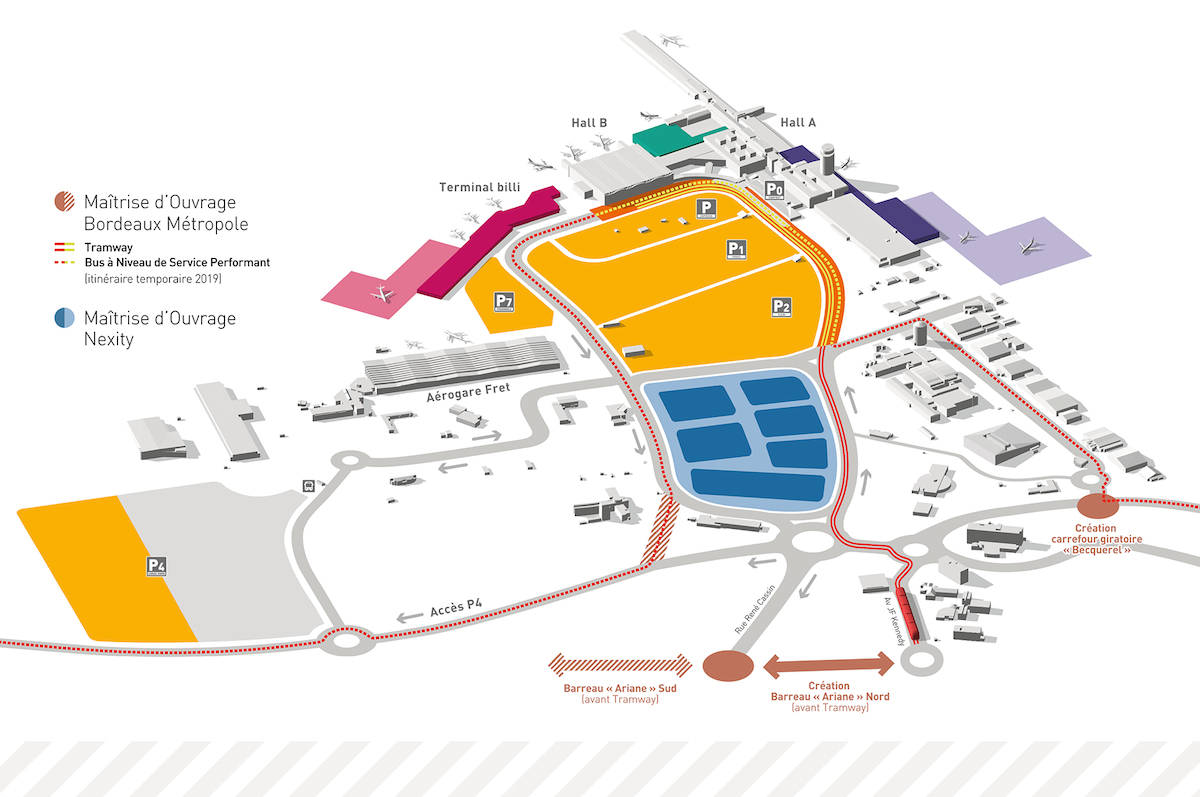
\includegraphics[width=16cm]{Images/tramway.jpg}
    \caption{Plan du futur tramway}
    \label{fig:futurtram}
\end{figure}

\newpage

\subsection{Ouverture sur le monde}

L'aéroport de Bordeaux-Mérignac est le 8ème aéroport français, 6ème hors région parisienne. Il sert de base à 4 compagnies : AirFrance, EasyJet, Ryanair et Volotea.\newline

Grâce à la plateforme aéroportuaire, près de 7,7 millions de passagers ont voyagé en 2019. Voici le détail des 10 destinations principales en 2019 :

\begin{table}[hbt!]
  \centering
  \begin{tabular}{|c|c|c|c|c|}
  \hline
  \textbf{Rang} & \textbf{Passagers} & \textbf{Destination}              & \textbf{Pays} & \textbf{Code IATA} \\ \hline
  \textbf{1}    & 1 217 787          & Paris (Orly et Charles-de-Gaulle) & France        & ORY/CDG            \\ \hline
  \textbf{2}    & 581 780            & Lyon-Saint-Exupéry                & France        & LYS                \\ \hline
  \textbf{3}    & 426 199            & Marseille-Provence                & France        & MRS                \\ \hline
  \textbf{4}    & 321 848            & Londres-Gatwick                   & Royaume-Uni   & LGW                \\ \hline
  \textbf{5}    & 298 245            & Amsterdam                         & Pays-Bas      & AMS                \\ \hline
  \textbf{6}    & 270 012            & Nice-Côte d'Azur                  & France        & NCE                \\ \hline
  \textbf{7}    & 244 610            & Lisbonne-H. Delgado               & Portugal      & LIS                \\ \hline
  \textbf{8}    & 227 641            & Lille Lesquin                     & France        & LIL                \\ \hline
  \textbf{9}    & 217 739            & Barcelone-El Prat                 & Espagne       & BCN                \\ \hline
  \textbf{10}   & 214 067            & Genève-Cointrin                   & Suisse        & GVA                \\ \hline
  \end{tabular}
\end{table}

Avant la pandémie de COVID-19, l'objectif était de faire voyager 10 millions de passagers en 2023.

Malheureusement, comme on peut le constater sur ce graphique, à cause de la pandémie le nombre de passagers a drastiquement chuté.\newline

\begin{figure}[hbt!]
  \centering
  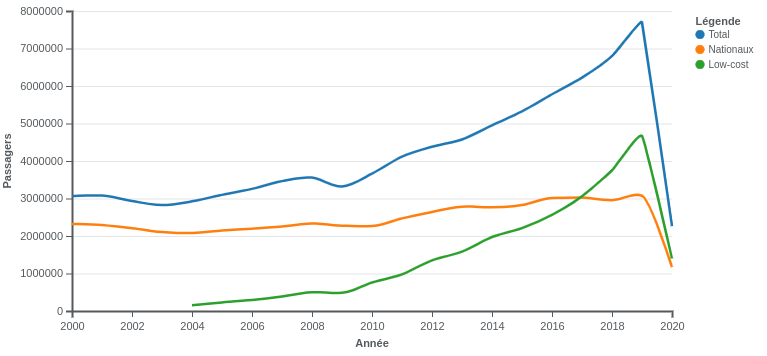
\includegraphics[width=16cm]{Images/passagers.png}
  \label{fig:trafic}
\end{figure}


En 2019, 34 compagnies aériennes ont opéré des vols sur la plateforme aéroportuaire, avec un total de 163 lignes directes reliées à 31 pays différents.

De plus, plus de 125 000 tonnes de fret ont été acheminées grâce aux vols cargos (UPS avec StarAir et DHL avec European Air Transport).

\begin{figure}[hbt!]
  \centering
  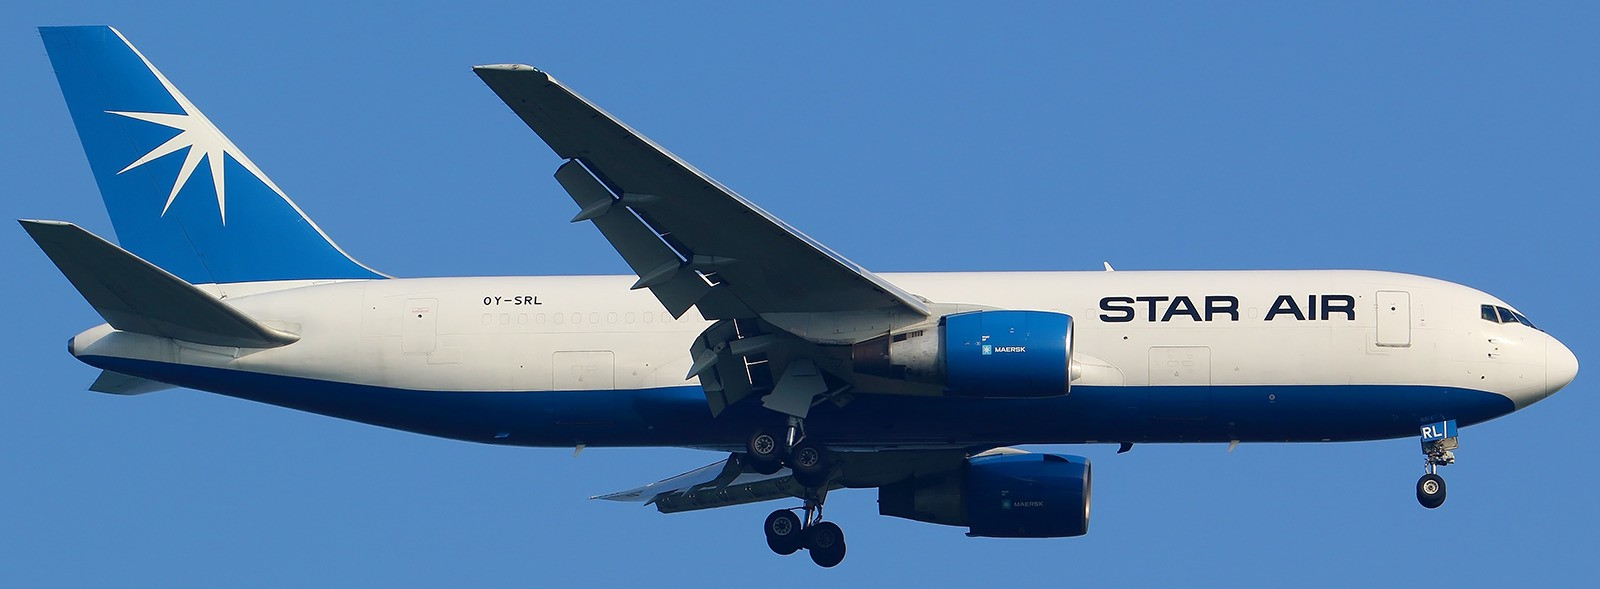
\includegraphics[width=7cm]{Images/starair.jpg}
  \caption{Avion StarAir}
  \label{fig:starair}
\end{figure}

C'est également un bassin d'emploi important puisque plus de 8000 personnes travaillent sur la plateforme aéroportuaire (dont 200 à la SA ADBM). 94 employeurs sont présents sur site : entreprises, commerces, industries, organismes publics et organismes d'état.

\newpage

\section{Personnes impliquées}


Mon tuteur était Monsieur Serge CLARY, Chef de Projet Informatique, et ma supérieure Madame Nathalie CORDEAU, Chef du Service Organisation, Informatique, Systèmes Industriels (SOISI) au sein du Département des Opérations Techniques (DOT)\footnote{Tous les organigrammes sont disponibles en annexe, page 21 et 22}.\newline

J'ai travaillé en proche collaboration avec :

\begin{itemize}
    \item Monsieur Gurvan QUENET : Responsable Sécurité des Systèmes d'Information,
    \item Monsieur Kamal MAHAMOUD : Technicien Support Informatique,
    \item Monsieur Marc RIVAULT : Administrateur Systèmes, Réseaux et Bases de données,
    \item Monsieur Nicolas PALAZON : Administrateur Systèmes, Réseaux et Bases de données,
    \item Monsieur Yannick FOURNAUD : Administrateur Systèmes, Réseaux et Bases de données.\newline
\end{itemize}

J'ai également été reçue par :

\begin{itemize}
    \item Madame Christelle DIJOUX : Chargée de Mission SMQS SME\footnote{Système de Management de l'Entreprise, essentiellement de la Qualité (SMQ), de l'Environnement (SME) et de la Sécurité (SMS)},
    \item Madame Fabienne COLAS : Coordinatrice Piste,
    \item Monsieur Olivier CABANNE : Attaché Relations Riverains et Environnement,
    \item Monsieur Yannick VALERY : Administrateur Systèmes, Réseaux et Bases de données.\newline
\end{itemize}

L'avantage d'une entreprise avec une grande variété de postes est que j'ai pu constater à quel point l'informatique est indispensable dans tous les services, autant sur l'aspect logiciel que matériel.

Je remercie également l'ensemble du personnel de la SA ADBM pour leur accueil et leur bienveillance. 

\section{Missions et tâches réalisées}

Plusieurs types de tâches m’ont été données, à la fois techniques mais également administratives :\

\subsection{Office}

Les salariés de l’aéroport travaillant toujours sur Office 2010, ma première mission a été d’analyser les différences entre Office 2010 et 2019 afin de savoir quel type de formation ou documentation pourrait accompagner la transition, et ensuite de réaliser les supports adéquats. J’ai donc créé un document détaillé de tous les changements entre ces versions, puis ensuite un flyer\footnote{Disponible en annexe page 23 et 24} les résumant de manière simplifiée.\newline


\begin{figure}[hbt!]
  \centering
  
\includegraphics[width=12cm]{Images/office.png}
  \caption{Suite Office 2019}
  \label{fig:office}
\end{figure}

\newpage


\subsection{Crews}

Ma seconde mission était de mettre à jour des ordinateurs "Crews" et de les passer de Windows 7 à Windows 10 en réinstallant d’autres logiciels.

Les banques d’enregistrements sont équipées de ces ordinateurs qui permettent d’enregistrer les bagages en soute et d’imprimer leurs identifications à partir d’un scan de la carte d’embarquement du passager. Ces mêmes matériels servent également pour l’accès au Poste Inspection Filtrage (PIF) et en porte d’embarquement. Les passagers scannent leur carte d’embarquement pour que le personnel aéroportuaire ait accès aux informations dont il a besoin pour procéder à ces derniers.

J’ai commencé à faire quelques manipulations sur les ordinateurs Crews : mise à jour du BIOS et installation de Windows à partir d’un logiciel de gestion appelé Ivanti. Cependant je n’ai jamais eu l'occasion de les installer car des complications techniques ont été repérées plus tard dans l’installation. Le projet a donc dû être temporairement suspendu.

\begin{figure}[hbt!]
  \begin{subfigure}{0.5\textwidth}
    \centering
    % include first image
    
\includegraphics[width=10cm]{Images/logocrews.png}  
    \label{fig:logocrews}
  \end{subfigure}
  \begin{subfigure}{0.5\textwidth}
    \centering
    % include second image
    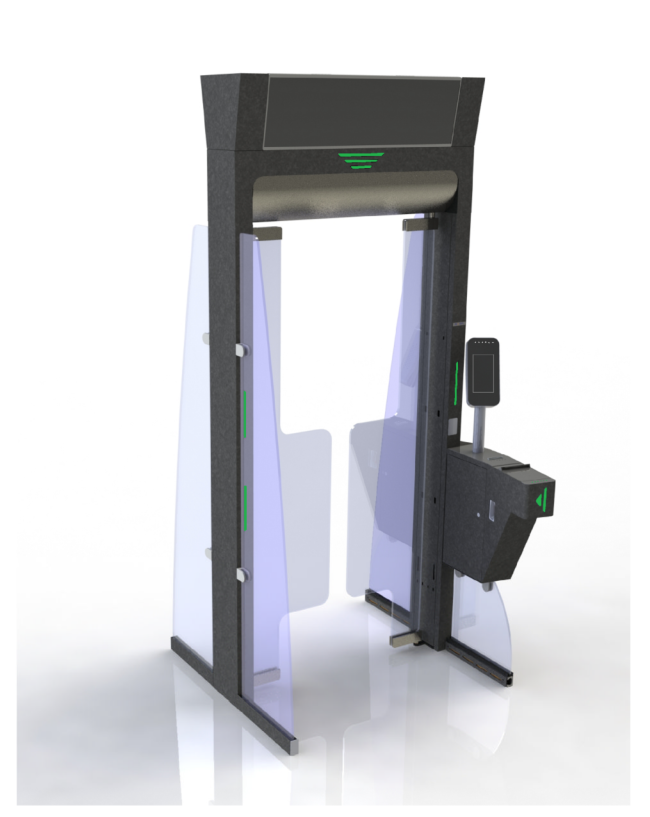
\includegraphics[width=6cm]{Images/crews2.png}\newline  
    \label{fig:portecrews}
  \end{subfigure}
  \caption{Crews en porte d'embarquement}
\end{figure}


\subsection{Wyse}

J’ai également dû intervenir sur les boîtiers Wyse. Ce matériel est utilisé à l’aéroport comme boîtiers de téléaffichage. Ils servent notamment à afficher les écrans de départs et d’arrivées des vols, les temps d’attente, les destinations sur les portes d’embarquements et banques d'enregistrements. Un modèle plus performant a été acheté et il fallait donc les configurer : mise à jour du BIOS, flash du BIOS, installation de Windows et installation dans le réseau.


J’ai donc effectué ces démarches sur une trentaine de postes.\newline

\begin{figure}[hbt!]
  \begin{subfigure}{0.5\textwidth}
    \centering
    % include first image
    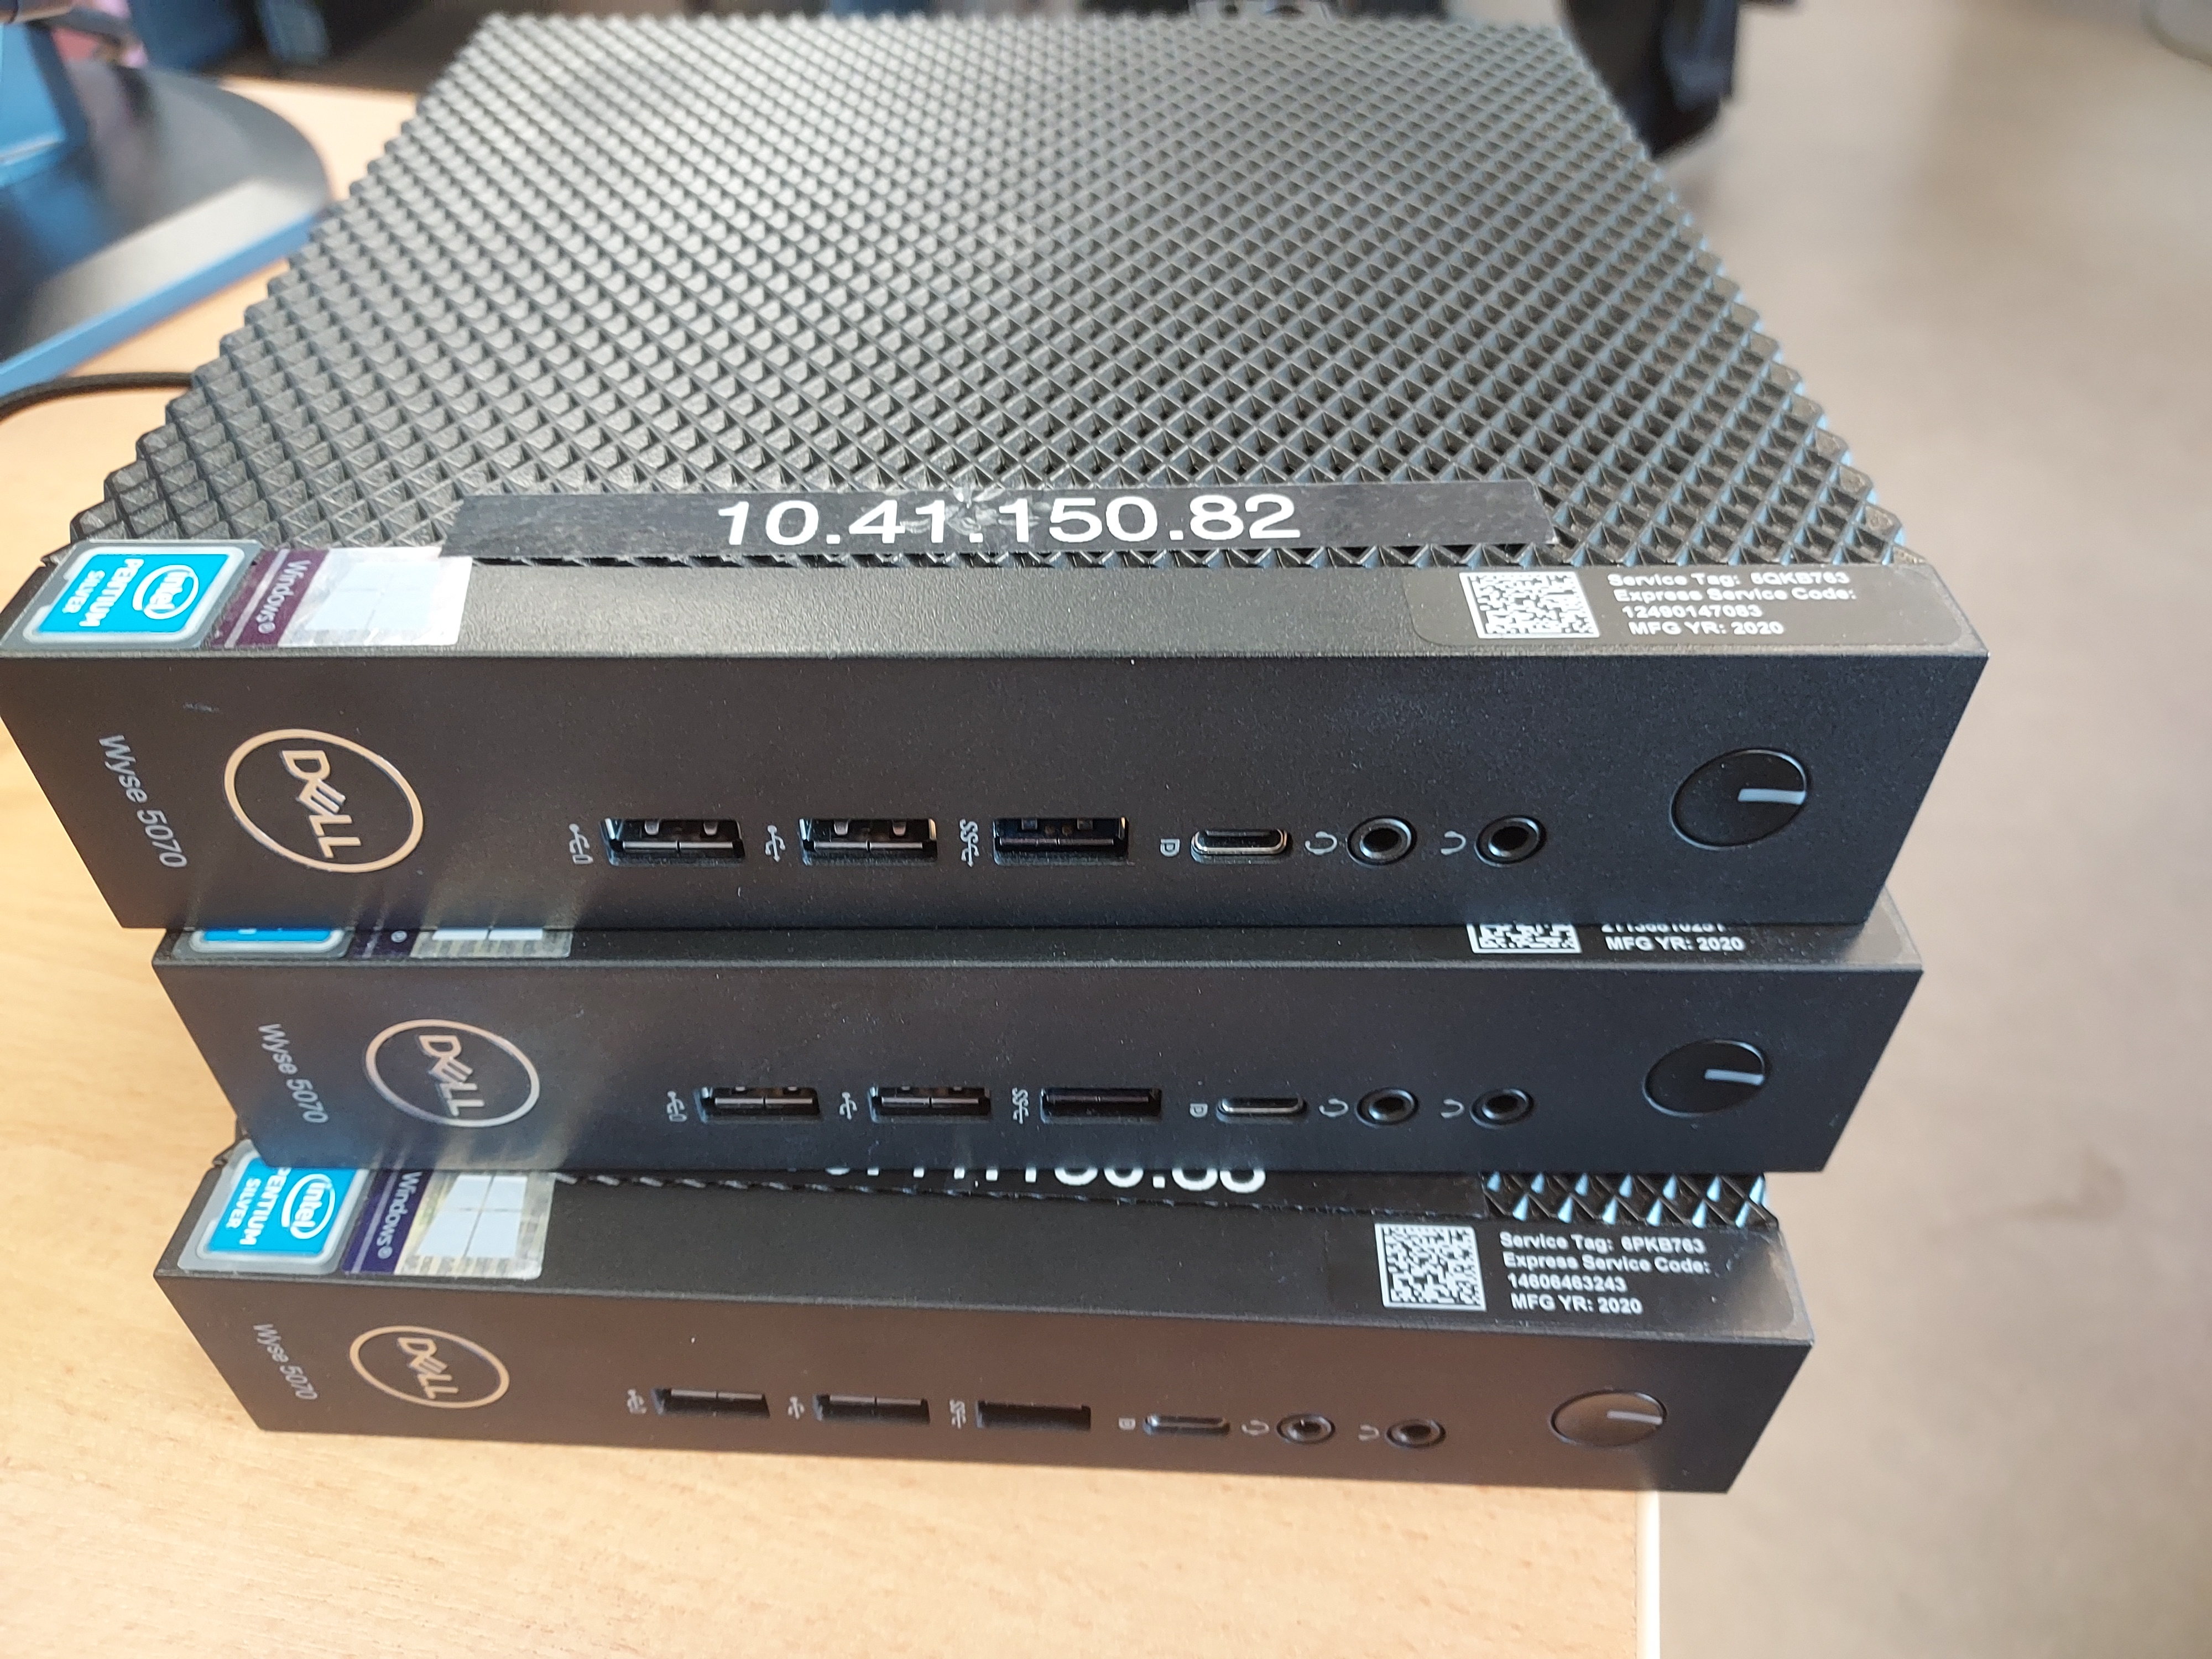
\includegraphics[width=7.2cm]{Images/wyse.jpg}  
    \label{fig:wyse}
  \end{subfigure}
  \begin{subfigure}{0.5\textwidth}
    \centering
    % include second image
    
\includegraphics[width=7.2cm]{Images/wyse_logo.jpg}  
    \label{fig:logowyse}
  \end{subfigure}
  \caption{Boîtiers Wyse}
\end{figure}

\subsection{Inventaire}

Durant le premier confinement, certains salariés se sont vus attribuer un ordinateur portable afin de faire du télétravail.

Une de mes missions était de passer dans tous les bureaux de l’aéroport pour recenser le matériel présent et des informations le concernant (modèle et numéro de série). Il m'a fallu ensuite comparer cette liste avec celle du matériel prêté afin de vérifier que tout le personnel avait bien ramené les outils mis à sa disposition.
Finalement, il m'a fallu produire un inventaire du matériel présent sur site.\newline

\subsection{CRYHOD}

Concernant ma dernière mission, il est apparu que plusieurs salariés se sont fait voler le matériel de l'entreprise. Au delà de la perte financière, la disparition du disque dur représentait une perte d’informations internes et donc un problème de sécurité. Il fallait donc régler le problème afin de ne pas risquer une fuite de données. Le Responsable Sécurité des Systèmes d’Information et ses supérieurs ont opté pour CRYHOD.


CRYHOD est un logiciel de cryptage de données de disques durs. Gurvan QUENET, le responsable cybersécurité de l’aéroport, m’a donc donné la mission d’installer ce logiciel sur les ordinateurs portables des salariés afin de sécuriser les disques durs et protéger les données de l’aéroport.\newline

J’ai pu effectuer cette installation sur les postes de mon service, mais je n'ai pas eu le temps de continuer sur ceux de l'ensemble du personnel. Sur la consigne de Monsieur Gurvan QUENET, j'ai donc dû, avant mon départ, former mon collègue Monsieur Kamal MAHAMOUD à cette installation afin qu'il la termine.\newline

\begin{figure}[hbt!]
  \centering
  
\includegraphics[width=10cm]{Images/logo_cryhod.png}
  \label{fig:logocryhod}
\end{figure}

\newpage

\section{Démarche Responsabilité Sociale (ou Sociétale) de l’Entreprise}


Lorsque l'on pense à un aéroport ou même au milieu aéronautique en général, on ne l'associe pas à une bonne gestion de l'environnement.
Et pourtant, comme toute entreprise, l'aéroport de Bordeaux-Mérignac pratique une démarche Responsabilité Sociale (ou Sociétale) de l'Entreprise (RSE).

J'ai pu rencontrer un des responsables du service environnement et relations riverains : Monsieur Olivier CABANNE, et la responsable du service qualité : Madame Christelle DIJOUX.\newline

En effet, l'entreprise se rend compte que ses activités sont des nuisances pour les riverains et l'environnement. 

La Commission Consultative de l’Environnement (CCE) est l’instance de référence consultée sur toute question d’importance relative à l’aménagement ou à l’exploitation de l’aéroport de Bordeaux pouvant avoir une incidence sur l’environnement. Ces réunions rassemblent : 

\begin{itemize}
  \item Le Service Environnements et Relations Territoriales de l'aéroport de Bordeaux-Mérignac,
  \item Les Élus Locaux,
  \item Les Associations de Riverains.
\end{itemize}

Suite à ces réunions, la SA ADBM propose de nombreuses solutions.\newline

\subsection{Riverains}

Plusieurs actions ont été menées afin de réduire au maximum la gêne occasionnée par les activités aériennes, comme la mise en place d'Aérovision.


\subsubsection{Aérovision}

\begin{figure}[hbt!]
  \centering
  
\includegraphics[width=2.3cm]{Images/logo_aerovision.jpg}
  \label{fig:logoaerovision}
\end{figure}

La majorité des plaintes sont relatives au bruit occasionné par les aéronefs qui volent à basse altitude afin d'atterir ou de décoller.
Ces bruits sont soumis à une loi : le bruit capté au sol ne doit pas dépasser les 70 dB. Plusieurs associations de riverains se plaignaient que certains avions dépassaient cette réglementation.\newline

Le service informatique a donc créé Aérovision. Des stations de mesure de bruit ont été installées dans des endroits habités dans l'axe des pistes.

Cet outil accessible en ligne est une carte de l'aéroport et de ses environs avec la représentation des stations ainsi que le bruit mesuré lorsqu'un avion passe au dessus. Les trajectoires vertes sont les arrivées, et les bleues sont les décollages.

\begin{figure}[hbt!]
  \centering
  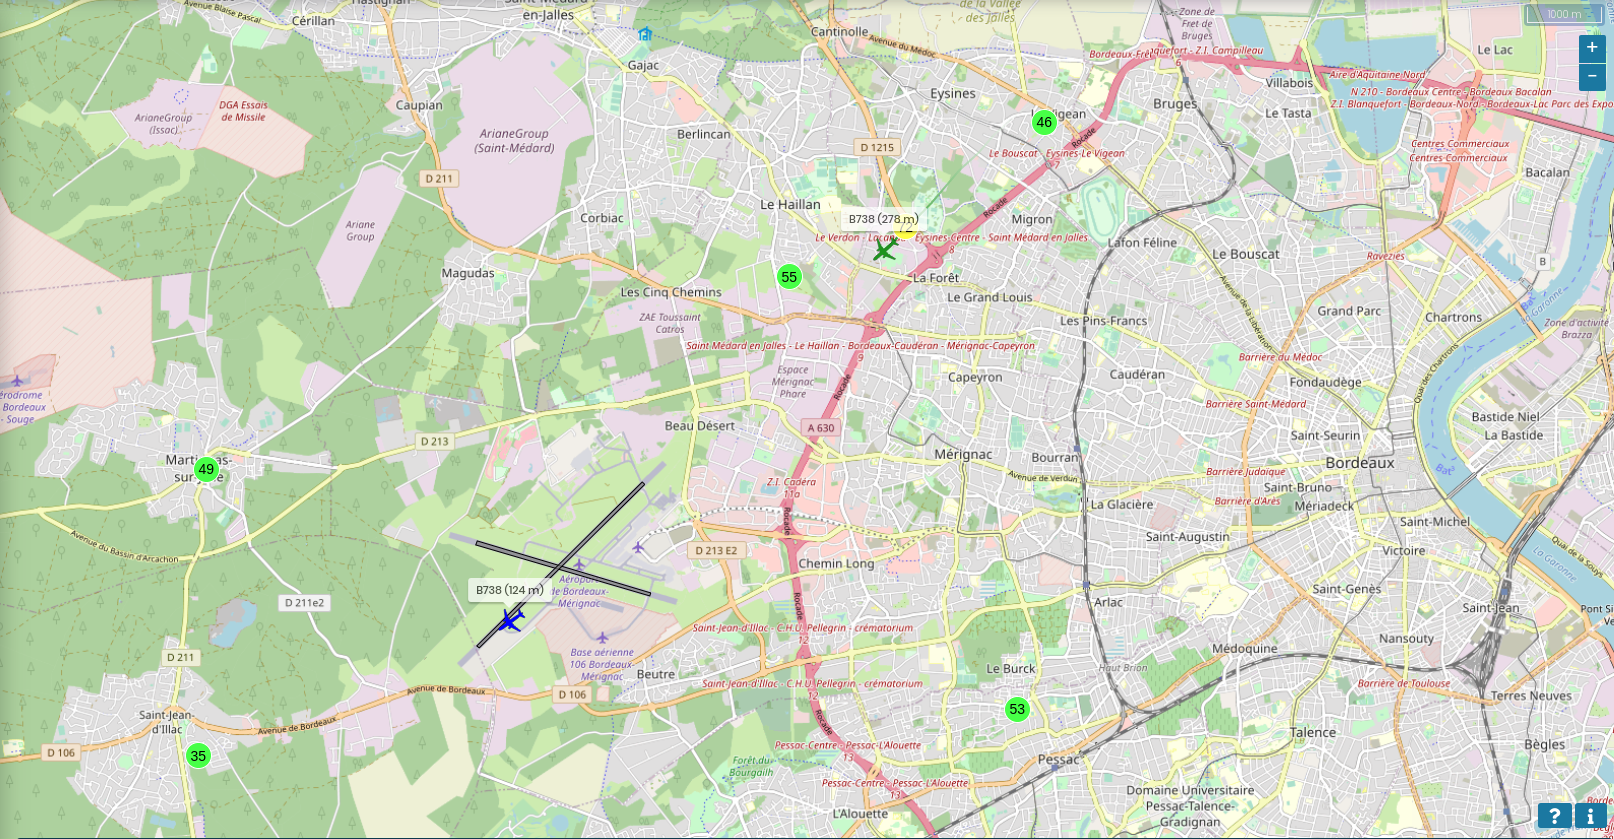
\includegraphics[width=15.4cm]{Images/aerovision.png}\newline
  \caption{Interface}
  \label{fig:interfaceaerovision}
\end{figure}

\newpage

Un mode "Historique" est également disponible : grâce à une sélection de 30 minutes, l'utilisateur peut vérifier les informations sur des vols antérieurs.

Pour des raisons de sûreté, Aérovision a 30 minutes de décalage avec la réalité et n'affiche que les vols civils.

L'outil Aérovision est disponible à l'adresse : https://trajectoires.bordeaux.aeroport.fr/appmap\newline

De plus, en cliquant sur un avion sur la carte, on peut obtenir des informations sur celui-ci : type d'appareil, compagnie, trajectoire, informations d'approche et bruit total.
Une autre fonctionnalité a été créé pour les riverains : "Mon Habitation". Elle permet de placer sa maison sur la carte grâce à la géolocalisation ou simplement en cliquant sur cette dernière et d'afficher le point de bruit maximum par rapport à l'habitation.

\begin{figure}[hbt!]
  \begin{subfigure}{0.5\textwidth}
    \centering
    % include first image
    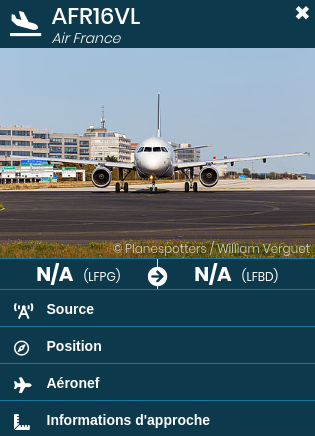
\includegraphics[width=5cm]{Images/aerovisioninfo.png}  
    \caption{Menu Informations Aéronefs}
    \label{fig:aerovisioninfo}
  \end{subfigure}
  \begin{subfigure}{0.5\textwidth}
    \centering
    % include second image
    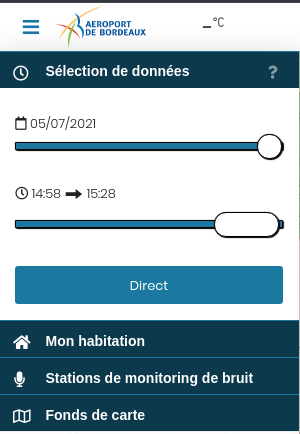
\includegraphics[width=5cm]{Images/aerovisionmaison.png}  
    \caption{Menu "Mon Habitation"}
    \label{fig:aerovisionmaison}
  \end{subfigure}
\end{figure}

\subsubsection{Aide à l'insonorisation}

Un dispositif d'aide a également été créé : l'aide à l'insonorisation.
C'est une aide financière destinée aux habitants des quatres communes touchées par ce problème : Mérignac, Le Haillan, Eysines et Saint-Jean-d'Illac. Elle prend en charge complètement les travaux de rénovation pour insonoriser l'hôtel, le local ou le logement.

Pour bénéficier de cette aide financière, il faut être situé dans une des zones du Plan de Gêne Sonore en vigueur, et avoir un permis de construire datant d'avant la création du Plan d'Exposition au Bruit\footnote{Les deux plans sont disponibles plus grands en annexe, page 25 et 26}.
Le but étant de dédommager les personnes s'étant installées près de l'aéroport avant l'augmentation signicative du trafic aérien.

\begin{figure}[hbt!]
  \centering
  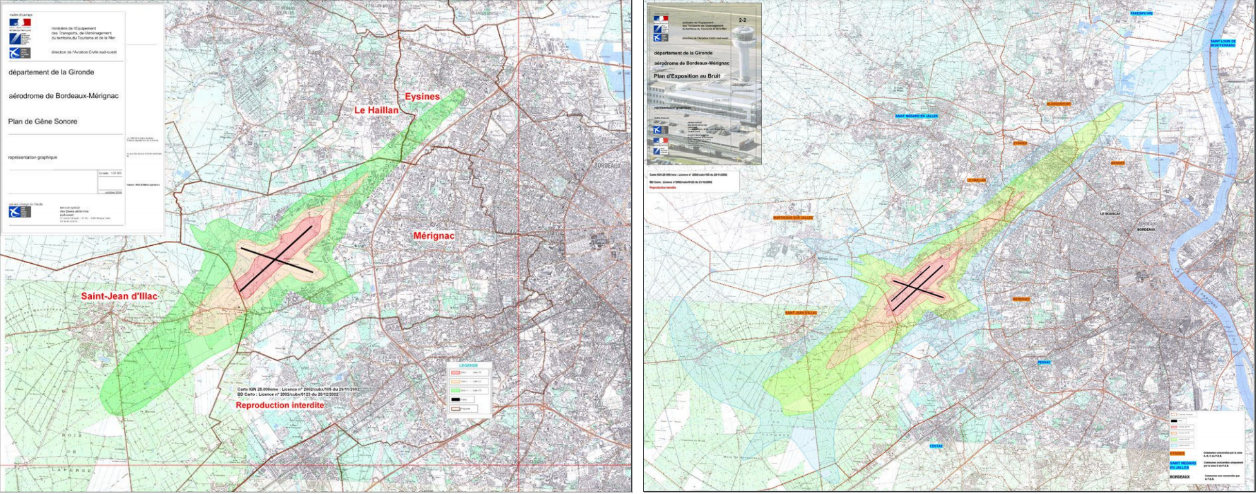
\includegraphics[width=16cm]{Images/pgs_peb.png}\newline
  \caption{Plan de Gêne Sonore et Plan d'Exposition au Bruit}
  \label{fig:pgs_peb}
\end{figure}

\subsubsection{Changement de trajectoire}

Une autre action a été effectuée pour les riverains : les quartiers de Pessac Toctoucau et Pierroton sont situés juste en dessous de la trajectoire de décollage de la piste la plus utilisée. Les riverains ont donc demandé à ce qu'un changement de trajectoire soit envisagé.

Le sujet a été longuement étudié et un obstacle majeur a été rencontré : si les aéronefs changeaient leurs trajectoires, ils devaient survoler une zone militaire, or cela est strictement interdit.
Une trajectoire alternative a toutefois été trouvée, mais il a ensuite fallu effectuer une demande aux services de l'état concernés. Celle-ci a été acceptée au bout d'un an et demi.\newline

Aujourd'hui, les avions remontant vers le nord effectuent leur virage bien plus au sud, et contournent donc les quartiers de Pierroton et de Toctoucau.\newline

\begin{figure}[hbt!]
  \centering
  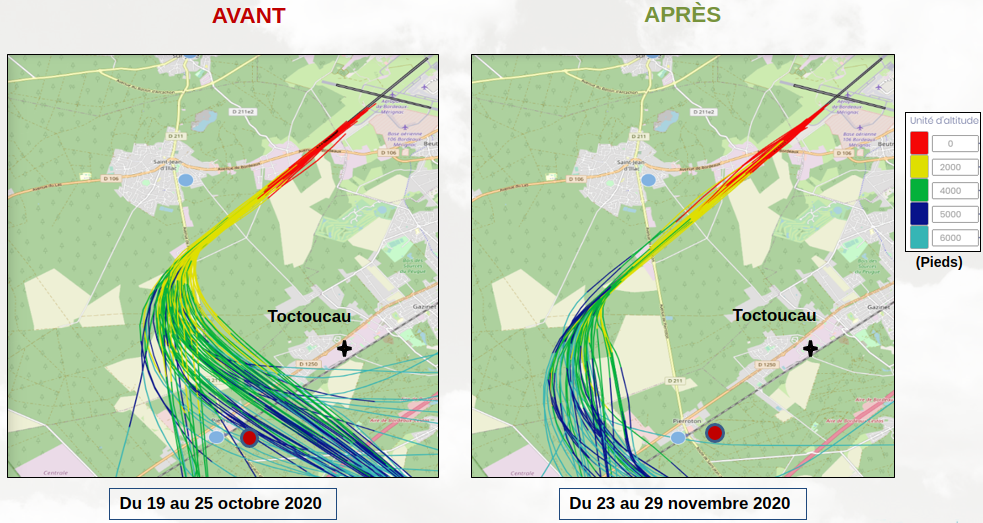
\includegraphics[width=13.5cm]{Images/trajectoires_avant_apres.png}\newline
  \caption{Différentes Trajectoires}
  \label{fig:trajectoires}
\end{figure}

Des mesures audios ont ensuite été réalisées sur les stations de bruit concernées afin de constater ou non des changements.

\begin{figure}[hbt!]
  \centering
  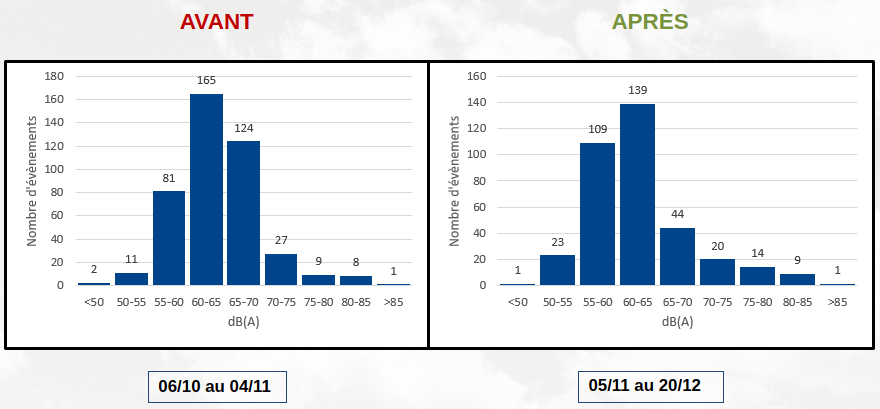
\includegraphics[width=14cm]{Images/bruit_avant_apres.png}\newline
  \label{fig:Mesures audios}
\end{figure}

De plus, pour répondre aux attentes des riverains, l'aéroport essaie de réduire les vols de nuit qui sont très gênants. Cependant ce n'est pas une tâche aisée puisque cela concerne également l'aéroport de destination ou de provenance du vol. Des discussions sont actuellement en cours avec certaines compagnies pour trouver des solutions pérennes qui satisferont l'ensemble des parties.\newline

\subsubsection{Bulletin d'information}

Une dernière action est menée pour améliorer la vie des riverains : trajectoires. C'est un bulletin d'information trimestriel\footnote{Exemplaire du premier trimestre 2021 disponible en annexe, page 27 et 28} qui leur est destiné dans lequel l'aéroport évoque les problématiques environnementales qui les concernent : mouvement des Rafales, statistiques sur les mesures de bruit, décollage et atterissage des aéronefs et qualité de l'air.


\subsection{Environnement}

Le milieu aérien est un domaine perçu comme très polluant par le grand public et la SA ADBM s'en rend compte. Un service est consacré à l'environnement. Ils travaillent sur différents points comme les émissions carbones, la faune et flore environnante mais également d'autres sujets.


Au niveau national, des lois ont été mises en place au niveau des compagnies aériennes. Par exemple, un passager peut s'il le souhaite choisir de compenser son émission carbone grâce à un don d'une valeur dépendant de la distance effectuée. Par exemple, sur un trajet Lille-Bordeaux, la compensation peut varier entre 2 et 8 euros.

Une partie de cet argent est par la suite utilisée pour acheter des avions moins polluants ou reversée aux aéroports afin de réduire les émissions de la plateforme.

\subsubsection{Consommation}

La SA ADBM prend ces enjeux très au sérieux : en effet, 8 millions d'euros ont été attribués pour réduire l'impact négatif sur l'environnement.
L'entreprise a également rejoint le programme Airport Carbon Accreditation (ACA). L'objectif de ce programme international est de rendre les plateformes aéroportuaires neutres en émissions carbone.
L'aéroport de Bordeaux-Mérignac a validé le niveau 1 le 11 juin 2021. L'objectif de neutralité carbone est prévu pour 2030\footnote{Les étapes du programme sont disponibles en annexe, page 29}.

\begin{figure}[hbt!]
  \centering
  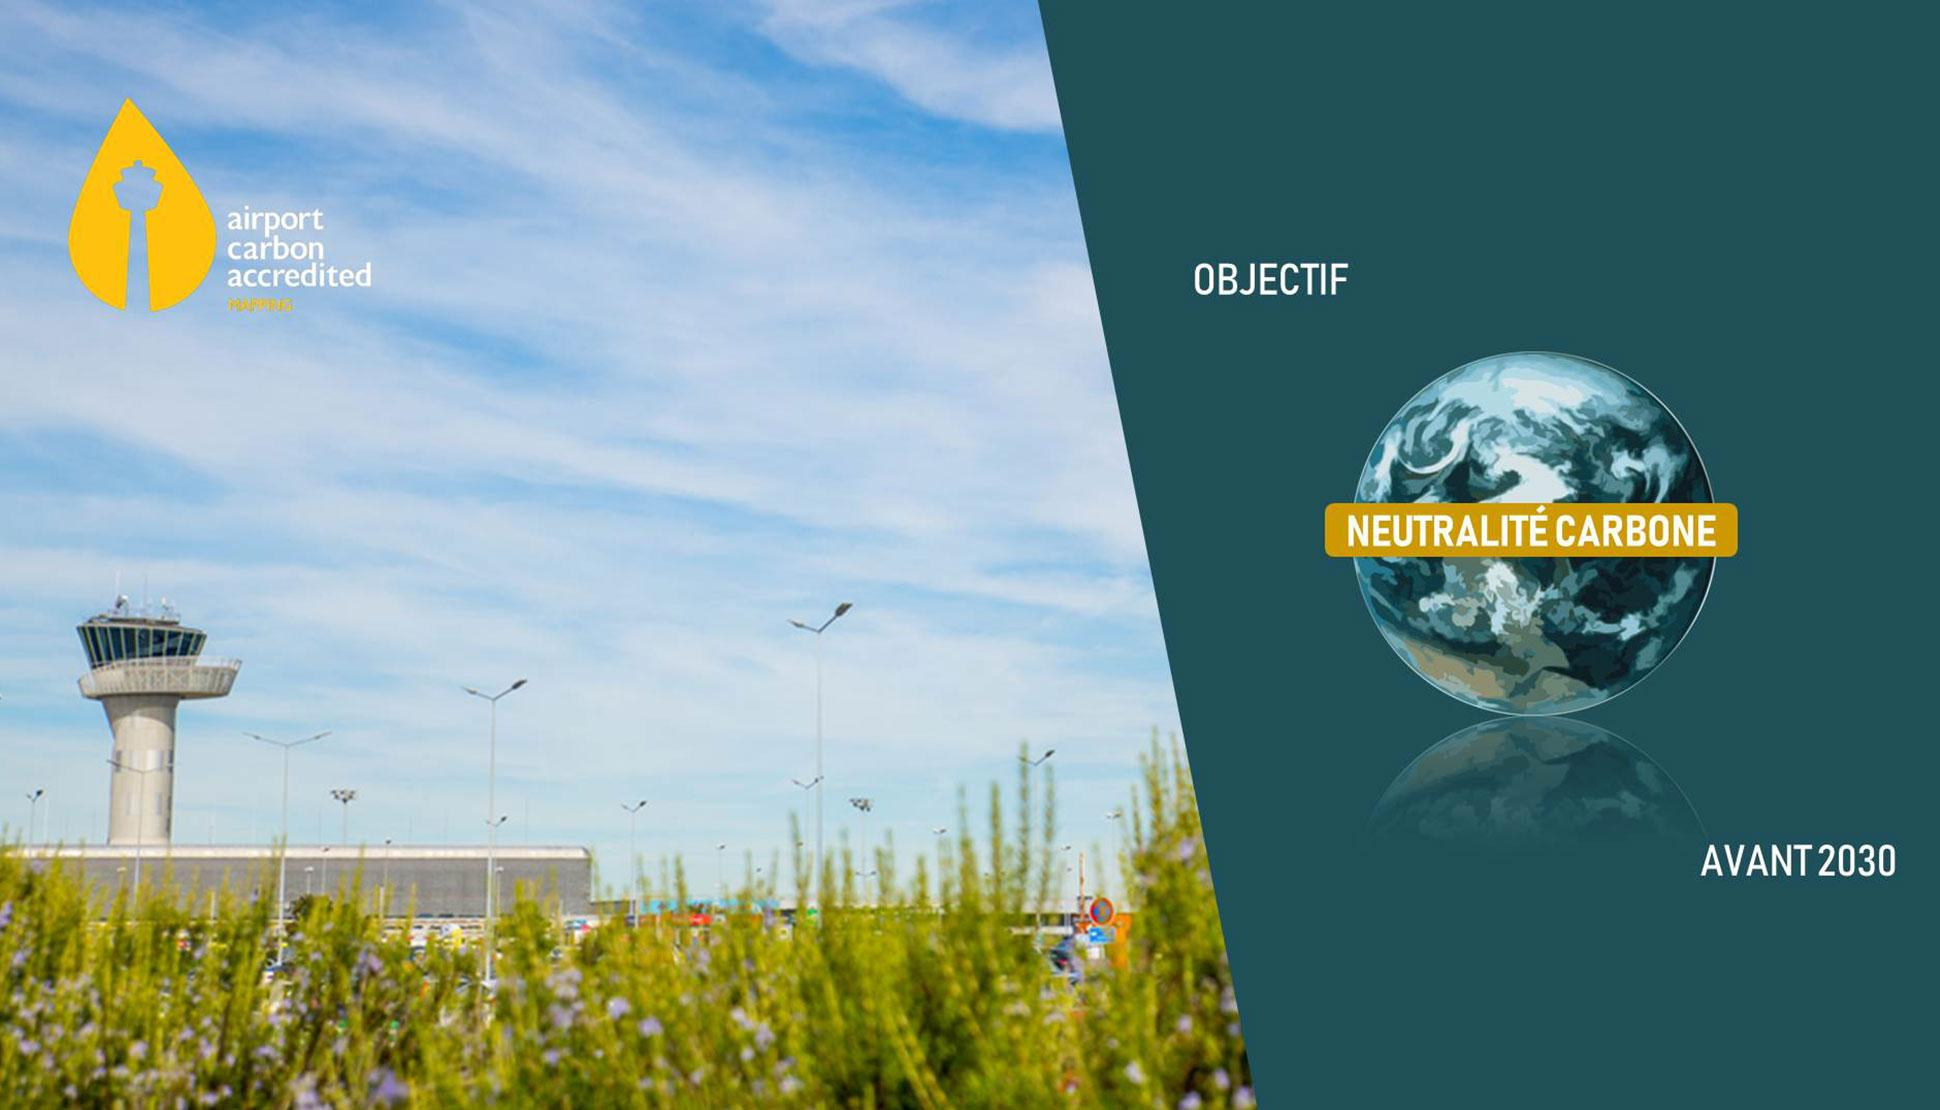
\includegraphics[width=9.5cm]{Images/aca2030.jpg}
  \caption{Airport Carbon Accreditation}
  \label{fig:aca2030}
\end{figure}


L'aéroport ne se limite pas à ce seul programme. Il a décidé d'agir de manière importante sur son activité afin de réduire leur pollution.


Concernant le côté ville, des actions comme le tri sélectif sont effectuées dans tout l'aéroport : pour le public mais également pour les salariés. La SA ADBM rembourse 80\% du prix de l'abonnement de transports en communs aux salariés si celui-ci sert à venir travailler, afin de lutter contre la pollution automobile.


La SA ADBM possède de nombreux véhicules : bus, voitures de services, voitures d'astreintes. Tous ces véhicules polluent et le service environnement de l'aéroport cherche à y remédier . Une nouvelle règle a été instaurée : lors d'un achat ou remplacement de véhicule, celui-ci doit être obligatoirement électrique ou hybride (selon les besoins). Cela permettra de réduire la consommation liée aux transports.\newline


Dans un objectif de réduction des émissions de carbone côté piste, la mise en place d’équipements d’alimentation électriques en « 400 Hertz » a été effectuée en remplacement des groupes électrogènes à moteur thermique. Ils servent notamment à maintenir l'alimentation électrique dans les aéronefs lorsqu'ils sont en escale.


De plus, tout nouveau bâtiment (comme le Satellite 3), doit être construit avec la norme Haute Qualité Environnementale et selon des critères renforcés de qualité de service. Cela permettra de réduire la consommation d'énergie sur le long terme.\newline


L'entreprise travaille également à la pose de panneaux photovoltaïques un peu partout sur la plateforme aéroportuaire : façades des Halls A et B, accès aux parkings et aux alentours des pistes.\newline


La plateforme aéroportuaire fait également attention à sa consommation d'eau. Des urinoirs secs ont été installés en 2019, et après 1 an ils ont permis d'économiser 1 million de litres d'eau. Leur installation continue donc progressivement.
De plus, la SA ADBM a un système de récupération de l'eau de pluie et des eaux servant à l'entraînement des pompiers de la plateforme.

\subsubsection{Faune et flore}

La végétalisation est un projet qui tient à coeur aux responsables environnement. Lors de l'arrivée du tramway en 2022, les abords seront végétalisés avec l'exigence « zéro phytosanitaire ».\newline


La faune et la flore sont des points très importants lors de l'évolution des infrastructures. Avant de lancer une construction, la SA ADBM fait intervenir un prestataire afin de réaliser une étude du terrain et étudier les conséquences sur l'environnement.
Concernant le projet "45ème Parallèle", c'est la société "Thallium" qui s'en est chargée. Ils étudient la faune et la flore locale et éditent un rapport sur ce qui doit être fait avant la construction.\newline

Voici une carte réalisée pour ce projet :

\begin{figure}[hbt!]
  \centering
  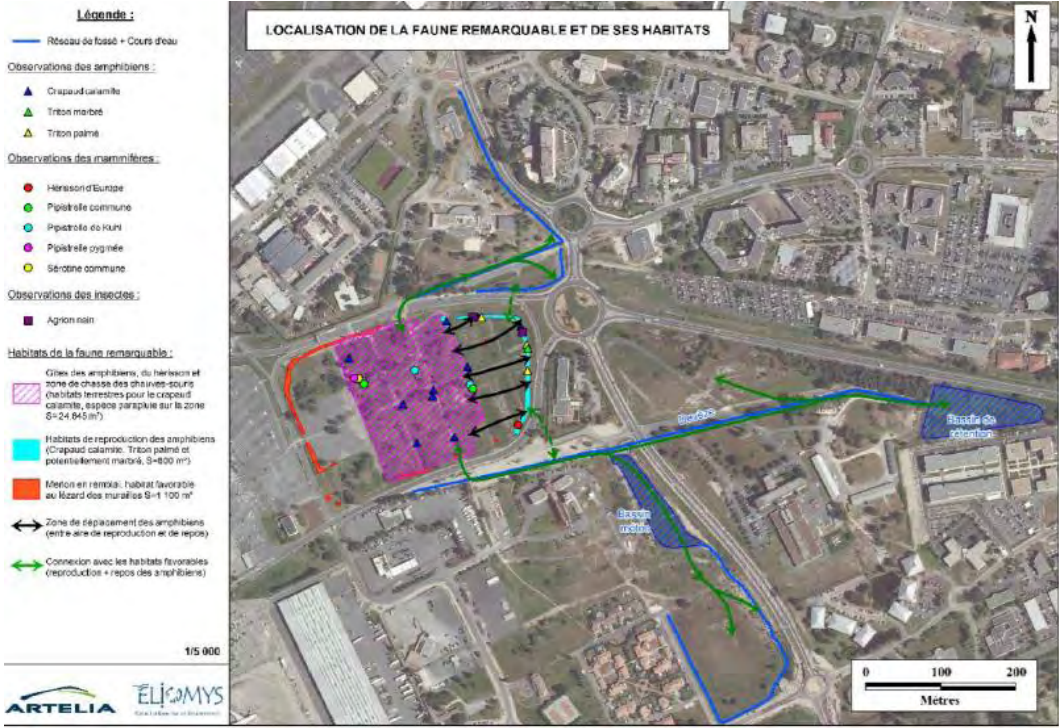
\includegraphics[width=13cm]{Images/carteenvironnement.png}
  \caption{Carte de localisation de la faune et de la flore}
  \label{fig:crapeau}
\end{figure}

La SA ADBM a également installé des ruches dans un endroit végétalisé éloigné de la vue du public. Une population de 150 000 abeilles s'y est installée. Un apiculteur vient régulièrement s'occuper des ruches et d'ici quelques mois, plusieurs kilogrammes de miel de l'aéroport de Bordeaux-Mérignac seront produits.

 \begin{figure}[hbt!]
   \centering
   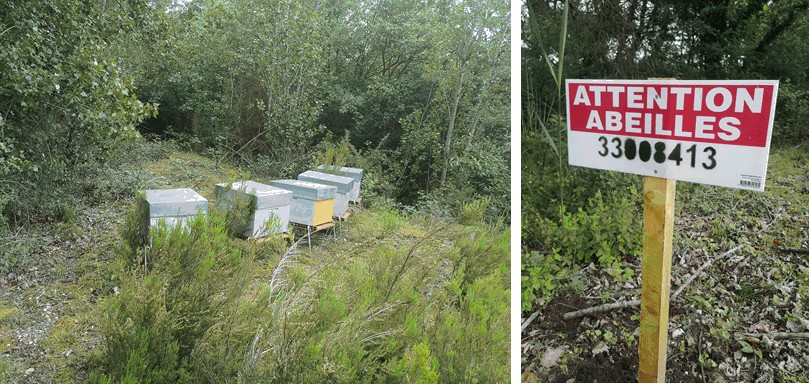
\includegraphics[width=10cm]{Images/ruches.jpg}
   \caption{Ruches}
   \label{fig:abeilles}
 \end{figure}


\end{document}

